\section{Problem set 1}
\subsection{Preface}

The goal of this problem set was a brief introduction to ,,VHDL'', a hardware
description language used in electronic design automation.

\subsection{Assignment 1}

This assignment consisted of a typical introduction task - writing
,,Hello world'' program using ,,VHDL'' as it was described in ,,GHDL Quick Start
Guide'' attached to assignment description. In this task I've interacted
with first lines of code in ,,VHDL'', I got to know basic structure of program
- not yet fully understood - and how does the flow of \textit{running} the
program looks like.

Process of compilation and execution of ,,VHDL'' program:
\begin{itemize}
  \item compilation
  \item elaboration
  \item run
\end{itemize}
As the process is quite complicated and requires to run three seperate commands,
that encouraged me to create a \texttt{Makefile} that I used when solving
assignments.

\subsection{Assignment 2}

In this task I've extended program provided in ,,Quick Start Guide'' using
functionality provided by \texttt{textio} library. The goal of this task was to
create program that interacts with \texttt{stdio} - reads a line and prints it
to the console.


\begin{lstlisting}[
  style=vhdl,
  caption={Code that reads line from standard input and prints it.},
  captionpos=b
]
  use std.textio.all;

  entity hello_world is
  end hello_world;


  architecture behaviour of hello_world is
  begin
     process
        variable l : line;
     begin
        write (l, String'("Hello world!"));
        writeline (output, l);
        readline (input, l);
        writeline (output, l);
        wait;
     end process;
  end behaviour;
\end{lstlisting}

\subsection{Assignment 3}

Here I've learned what are the basic ,,VHDL'' entities - what is required for
a valid ,,VHDL'' program:
\begin{enumerate}
  \item entity - the most basic building block in ,,VHDL''.
\begin{lstlisting}[
  style=vhdl,
  captionpos=b
  ]
  entity heartbeat is
    port ( clk: out std_logic );
  end heartbeat;
\end{lstlisting}
  \item architecture - description of entity's behaviour.
\begin{lstlisting}[style=vhdl, captionpos=b]
  architecture behaviour of heartbeat is
  constant clk_period : time := 10 ns;
  begin
    clk_process: process
    begin
      clk <= '0';
      wait for clk_period/2;
      clk <= '1';
      wait for clk_period/2;
    end process;
  end behaviour;
\end{lstlisting}
  \item port - definition of in and out connections to the entity.
  \begin{lstlisting}[style=vhdl]
  port ( clk: out std_logic );
  \end{lstlisting}
  \item component - in the testbench, or more generally, in external entity,
        is a definition of expected ports from another entity, for e. g.
        in testbench, component statement contained definition of how the
        tested entity looks like - what are it's expected ports.
  \begin{lstlisting}[style=vhdl]
  component logic_gate
    port (a : in bit; b : in bit; c : in bit; x : out bit);
  end component;
  \end{lstlisting}
  \item process - basic unit of execution in ,,VHDL'', part of \texttt{architecture}.
  \begin{lstlisting}[style=vhdl]
    process
      -- Process content definitions part here.
    begin
      -- Process flow definitions here.
    end process;
    \end{lstlisting}
\end{enumerate}

I also learned the basics about testing - how to create and use testbenches
for created entities and how to analyze tests output - using \textit{gtkwave}.
I've interacted with simple program and it's testbench.

\subsection{Assignment 4}

This problem was a sum up of all previous tasks. The goal here was to create
an entity that using three input ports, called \texttt{A}, \texttt{B} and
\texttt{C} calculated output values \texttt{X} and \texttt{Y} defined on
Figure \ref{fig:assignment4-gates}.

\begin{figure}[!htb]
  \center{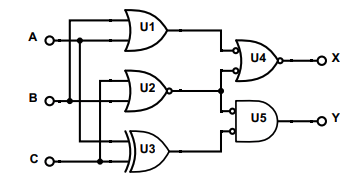
\includegraphics[scale=0.4]
  {drawings/gates.png}}
  \caption{\label{fig:assignment4-gates} Gates definition for assignment 4}
\end{figure}

After analysis of gates definition, all the gates were simplified to this flow:

$$ x \leftarrow \neg (\neg(a \lor b) \lor (b \lor c)) $$
$$ y \leftarrow (b \lor c) \land \neg(a \oplus c) $$

A corresponding ,,VHDL'' entity was created, code from entity was added on
listing \ref{fig:assignment4-code}.

\begin{lstlisting}[
  style=vhdl,
  caption={Implementation of logic gates from assignment 4},
  captionpos=b,
  label={fig:assignment4-code}
]
  entity logic_gate is
    port (a, b, c : in bit; x, y : out bit);
  end logic_gate;

  architecture rtl of logic_gate is
  begin
      x <= not(not(a or b) or (b or c));
      y <= (b or c) and not(a xor c);
  end rtl;
\end{lstlisting}

Created entity had been tested using testbench. A logic table was created
and output generated using created entity was compared to expected values.
Logic table in testbench was a vector of vectors with all possible
inputs combinations and expected outputs. For each vector in \texttt{pattern\_array},
first three elements were input \texttt{a, b, c} bits and last two elements
were expected \texttt{x, y} outputs. Listing \ref{fig:assignment4-testcode}
is a snippet of part of testbench with logic table definition.


\begin{lstlisting}[
  style=vhdl,
  caption={Part of code of entity testbench with logic table definition.},
  captionpos=b,
  label={fig:assignment4-testcode}
]
  constant patterns : pattern_array := (
    ('0', '0', '0', '0', '0'),
    ('0', '0', '1', '0', '0'),
    ('0', '1', '0', '0', '1'),
    ('0', '1', '1', '0', '0'),
    ('1', '0', '0', '1', '0'),
    ('1', '0', '1', '0', '1'),
    ('1', '1', '0', '0', '0'),
    ('1', '1', '1', '0', '1'));
\end{lstlisting}